\documentclass[12pt,a4paper]{article}
\usepackage[T1]{fontenc}
\usepackage[utf8]{inputenc}
\usepackage[brazil]{babel}
\usepackage{newtxtext,newtxmath}
\usepackage[scaled=0.92]{helvet}
\usepackage[a4paper,top=3.5cm,bottom=2.5cm,left=3cm,right=3cm]{geometry}
\usepackage{graphicx,float,array,tabularx,longtable,booktabs}
\usepackage[font={small,bf,sf},labelsep=period,skip=6pt,justification=centering]{caption}
\usepackage[table]{xcolor}
\usepackage{titlesec,enumitem,listings}
\usepackage[hidelinks]{hyperref}
\usepackage{xurl}

\titleformat{\section}{\fontsize{13}{15}\selectfont\bfseries}{\thesection.}{0.4em}{}
\titleformat{\subsection}{\fontsize{12}{14}\selectfont\bfseries}{\thesubsection.}{0.4em}{}
\titlespacing*{\section}{0pt}{12pt}{6pt}
\titlespacing*{\subsection}{0pt}{9pt}{4pt}
\setlength{\parindent}{1.27cm}
\setlength{\parskip}{0pt}
\renewcommand{\arraystretch}{1.3}
\newcommand{\rowsep}{\arrayrulecolor{black!18}\midrule\arrayrulecolor{black}}
\setlist{nosep,leftmargin=1.2cm}
\newcolumntype{Y}{>{\raggedright\arraybackslash}X}
\newcolumntype{L}[1]{>{\raggedright\arraybackslash}p{#1}}

\lstset{basicstyle=\ttfamily\scriptsize,columns=fullflexible,breaklines=true,
  keepspaces=true,showstringspaces=false,frame=single,rulecolor=\color{gray!60},commentstyle=\itshape\color{gray!70!black},
  keywordstyle=\bfseries,language=SQL,morekeywords={FILTER,WITHIN,ROLLUP,OVER,PARTITION,COMMENT,REFERENCES},
  literate={á}{{\'a}}1 {à}{{\`a}}1 {â}{{\^a}}1 {ã}{{\~a}}1 {é}{{\'e}}1 {ê}{{\^e}}1 {í}{{\'i}}1
           {ó}{{\'o}}1 {ô}{{\^o}}1 {õ}{{\~o}}1 {ú}{{\'u}}1 {ç}{{\c c}}1 {Ç}{{\c C}}1 {É}{{\'E}}1 {Ã}{{\~A}}1}

\begin{document}

\begin{center}
{\fontsize{16}{19}\selectfont\bfseries Atendimento de iluminação pública: análise das solicitações\\ do Recife\par}
\vspace{12pt}
{\bfseries Luís Henrique, Alan Vitor e Kaique William\par}
\vspace{6pt}
Universidade do Estado da Bahia (UNEB)\par
\vspace{6pt}
{\small Relatório final -- Tópicos Especiais em Banco de Dados -- 06/11/2026\par}
\end{center}

\section{Introdução}

Os registros de atendimento da iluminação pública do Recife são publicados pela Central 156 em um arquivo CSV, o que permite acompanhar o serviço a partir de dados abertos. No entanto, a análise desse arquivo exige organizar e relacionar os dados, de modo a identificar a concentração de solicitações por bairro e serviço e, ao mesmo tempo, comparar a situação publicada com o intervalo até o atendimento registrado.

Para isso, a solução proposta é um banco de dados relacional com carga reproduzível, acompanhado de um modelo multidimensional. Sobre esse banco foram construídas consultas para os níveis operacional, tático e estratégico, além de uma análise de mineração de dados e de um plano de ação, cujo objetivo comum é apoiar a escolha de ruas e bairros para manutenção preventiva.

A proposta se relaciona às metas 11.3 e 11.7 do Objetivo de Desenvolvimento Sustentável 11 (ODS 11), que tratam da gestão urbana e do acesso a espaços públicos [Ipea 2026]. Afinal, a iluminação faz parte das condições de uso de ruas e praças, de modo que as informações de atendimento permitem estudar esse serviço. Ainda assim, essas informações não medem os indicadores oficiais das metas e tampouco demonstram efeitos sobre segurança, consumo de energia ou emissões.

\section{Dados e requisitos}

Os dados vêm do CSV da Central 156 da Autarquia de Manutenção e Limpeza Urbana do Recife (EMLURB) [Emlurb 2026], disponível no portal de dados abertos municipal sob a licença Open Database License (ODbL) [Recife 2026]. O recorte reúne 34.492 registros do grupo ILUMINACAO PUBLICA com demandas abertas de 01/01 a 31/08/2025, distribuídos por 93 bairros, seis regiões político-administrativas (RPAs), dez serviços e cinco situações. Como o arquivo foi baixado diretamente em 18/10/2026, sem scraping, um manifesto documenta a origem, as transformações e o hash SHA-256 que identifica a versão utilizada.

A partir desse recorte, foram definidos os requisitos funcionais (RF) do sistema, apresentados na Tabela~\ref{tab:rf}.

\begin{table}[H]
\centering\small
\caption{Requisitos funcionais.}\label{tab:rf}
\begin{tabularx}{\textwidth}{lY}
\toprule
\textbf{Código} & \textbf{Descrição} \\ \midrule
RF01 & Importar o recorte de iluminação pública e registrar a origem dos dados. \\ \rowsep
RF02 & Relacionar RPA, bairro, grupo de serviço, serviço, situação e solicitação. \\ \rowsep
RF03 & Preservar o endereço e as datas de abertura e de última situação. \\ \rowsep
RF04 & Rejeitar chaves duplicadas, referências inexistentes e datas invertidas. \\ \rowsep
RF05 & Consultar volume e situação por bairro, RPA, serviço e mês de abertura. \\ \rowsep
RF06 & Calcular o intervalo até a última situação, separando ATENDIDA das demais. \\ \rowsep
RF07 & Refazer a carga analítica com o mesmo conteúdo a partir da fonte selecionada. \\ \rowsep
RF08 & Ordenar as ruas pela chance de nova solicitação nos dias seguintes, para priorizar inspeções. \\ \rowsep
RF09 & Agrupar os bairros por perfil de demanda e atendimento. \\ \bottomrule
\end{tabularx}
\end{table}

Por outro lado, o cadastro de cidadãos, equipes e ordens de serviço, o inventário de postes e a previsão de defeitos por poste ficam fora do escopo, uma vez que a fonte não contém essas informações.

\section{Modelagem dos dados}

O modelo transacional (OLTP, Online Transaction Processing) tem seis entidades, mostradas na Figura~\ref{fig:oltp}. Nele, a RPA reúne bairros, enquanto \textit{grupo\_servico} reúne os tipos de serviço. A entidade \textit{solicitacao}, por sua vez, associa bairro, serviço e situação ao endereço e às datas da demanda, e o cadastro de situações contém os estados publicados pela fonte. Como o recorte abrange apenas iluminação, \textit{grupo\_servico} tem um único registro, mas todos esses domínios existem no CSV.

\begin{figure}[H]
\centering
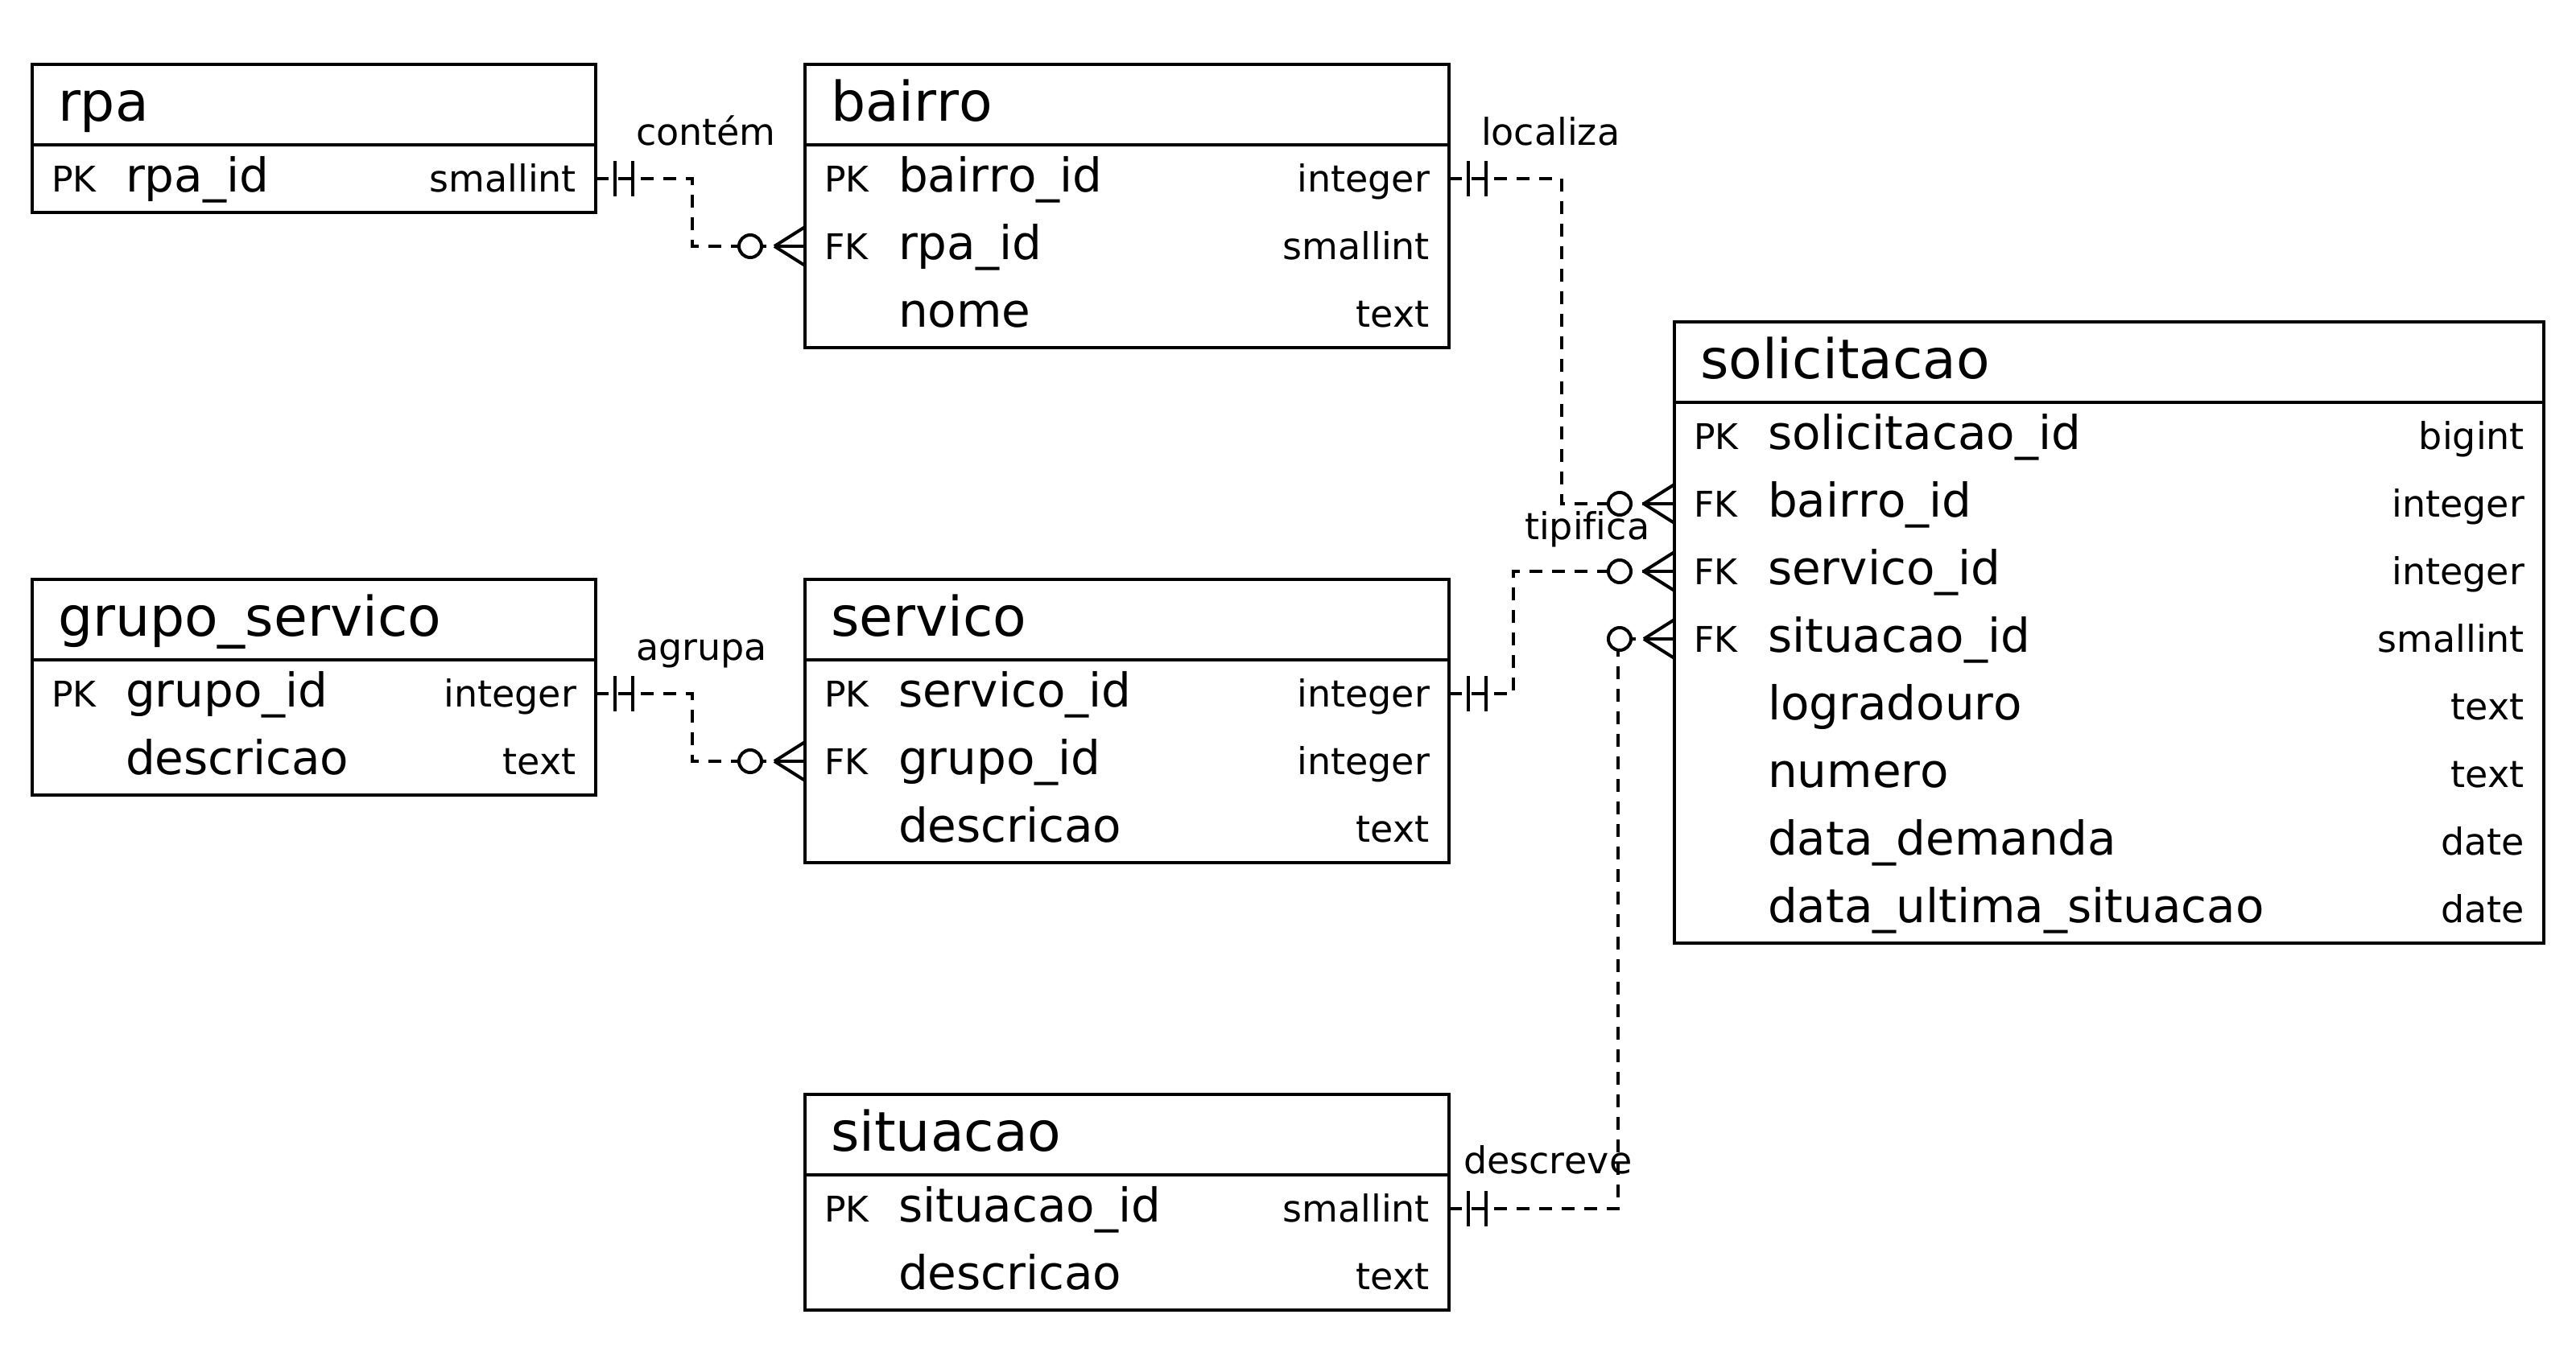
\includegraphics[width=0.92\textwidth]{../docs/diagrams/oltp_model.png}
\caption{Diagrama entidade-relacionamento (DER) do modelo OLTP.}\label{fig:oltp}
\end{figure}

Como o CSV não contém protocolo público, \textit{solicitacao\_id} usa a posição da linha de dados no arquivo original, identificado pelo hash, e por isso a chave vale apenas nessa versão. Além disso, o banco armazena somente a última situação disponível, sem criar etapas de atendimento que a fonte não informa, enquanto as restrições SQL rejeitam datas invertidas, chaves duplicadas e referências a cadastros inexistentes.

O modelo analítico (OLAP, Online Analytical Processing), por sua vez, segue um esquema estrela com um registro na tabela fato para cada solicitação publicada (Figura~\ref{fig:olap}). As quatro dimensões são data, bairro, serviço e situação, sendo que a dimensão de data é usada em dois papéis: abertura da demanda e última situação. Para simplificar as consultas, a RPA passa a ser um atributo de bairro, e o grupo, um atributo de serviço. Por fim, a fato contém a quantidade, fixada em 1 por registro, e o intervalo em dias entre a demanda e a última situação, que só é interpretado como prazo até o atendimento quando a situação é ATENDIDA.

\begin{figure}[H]
\centering
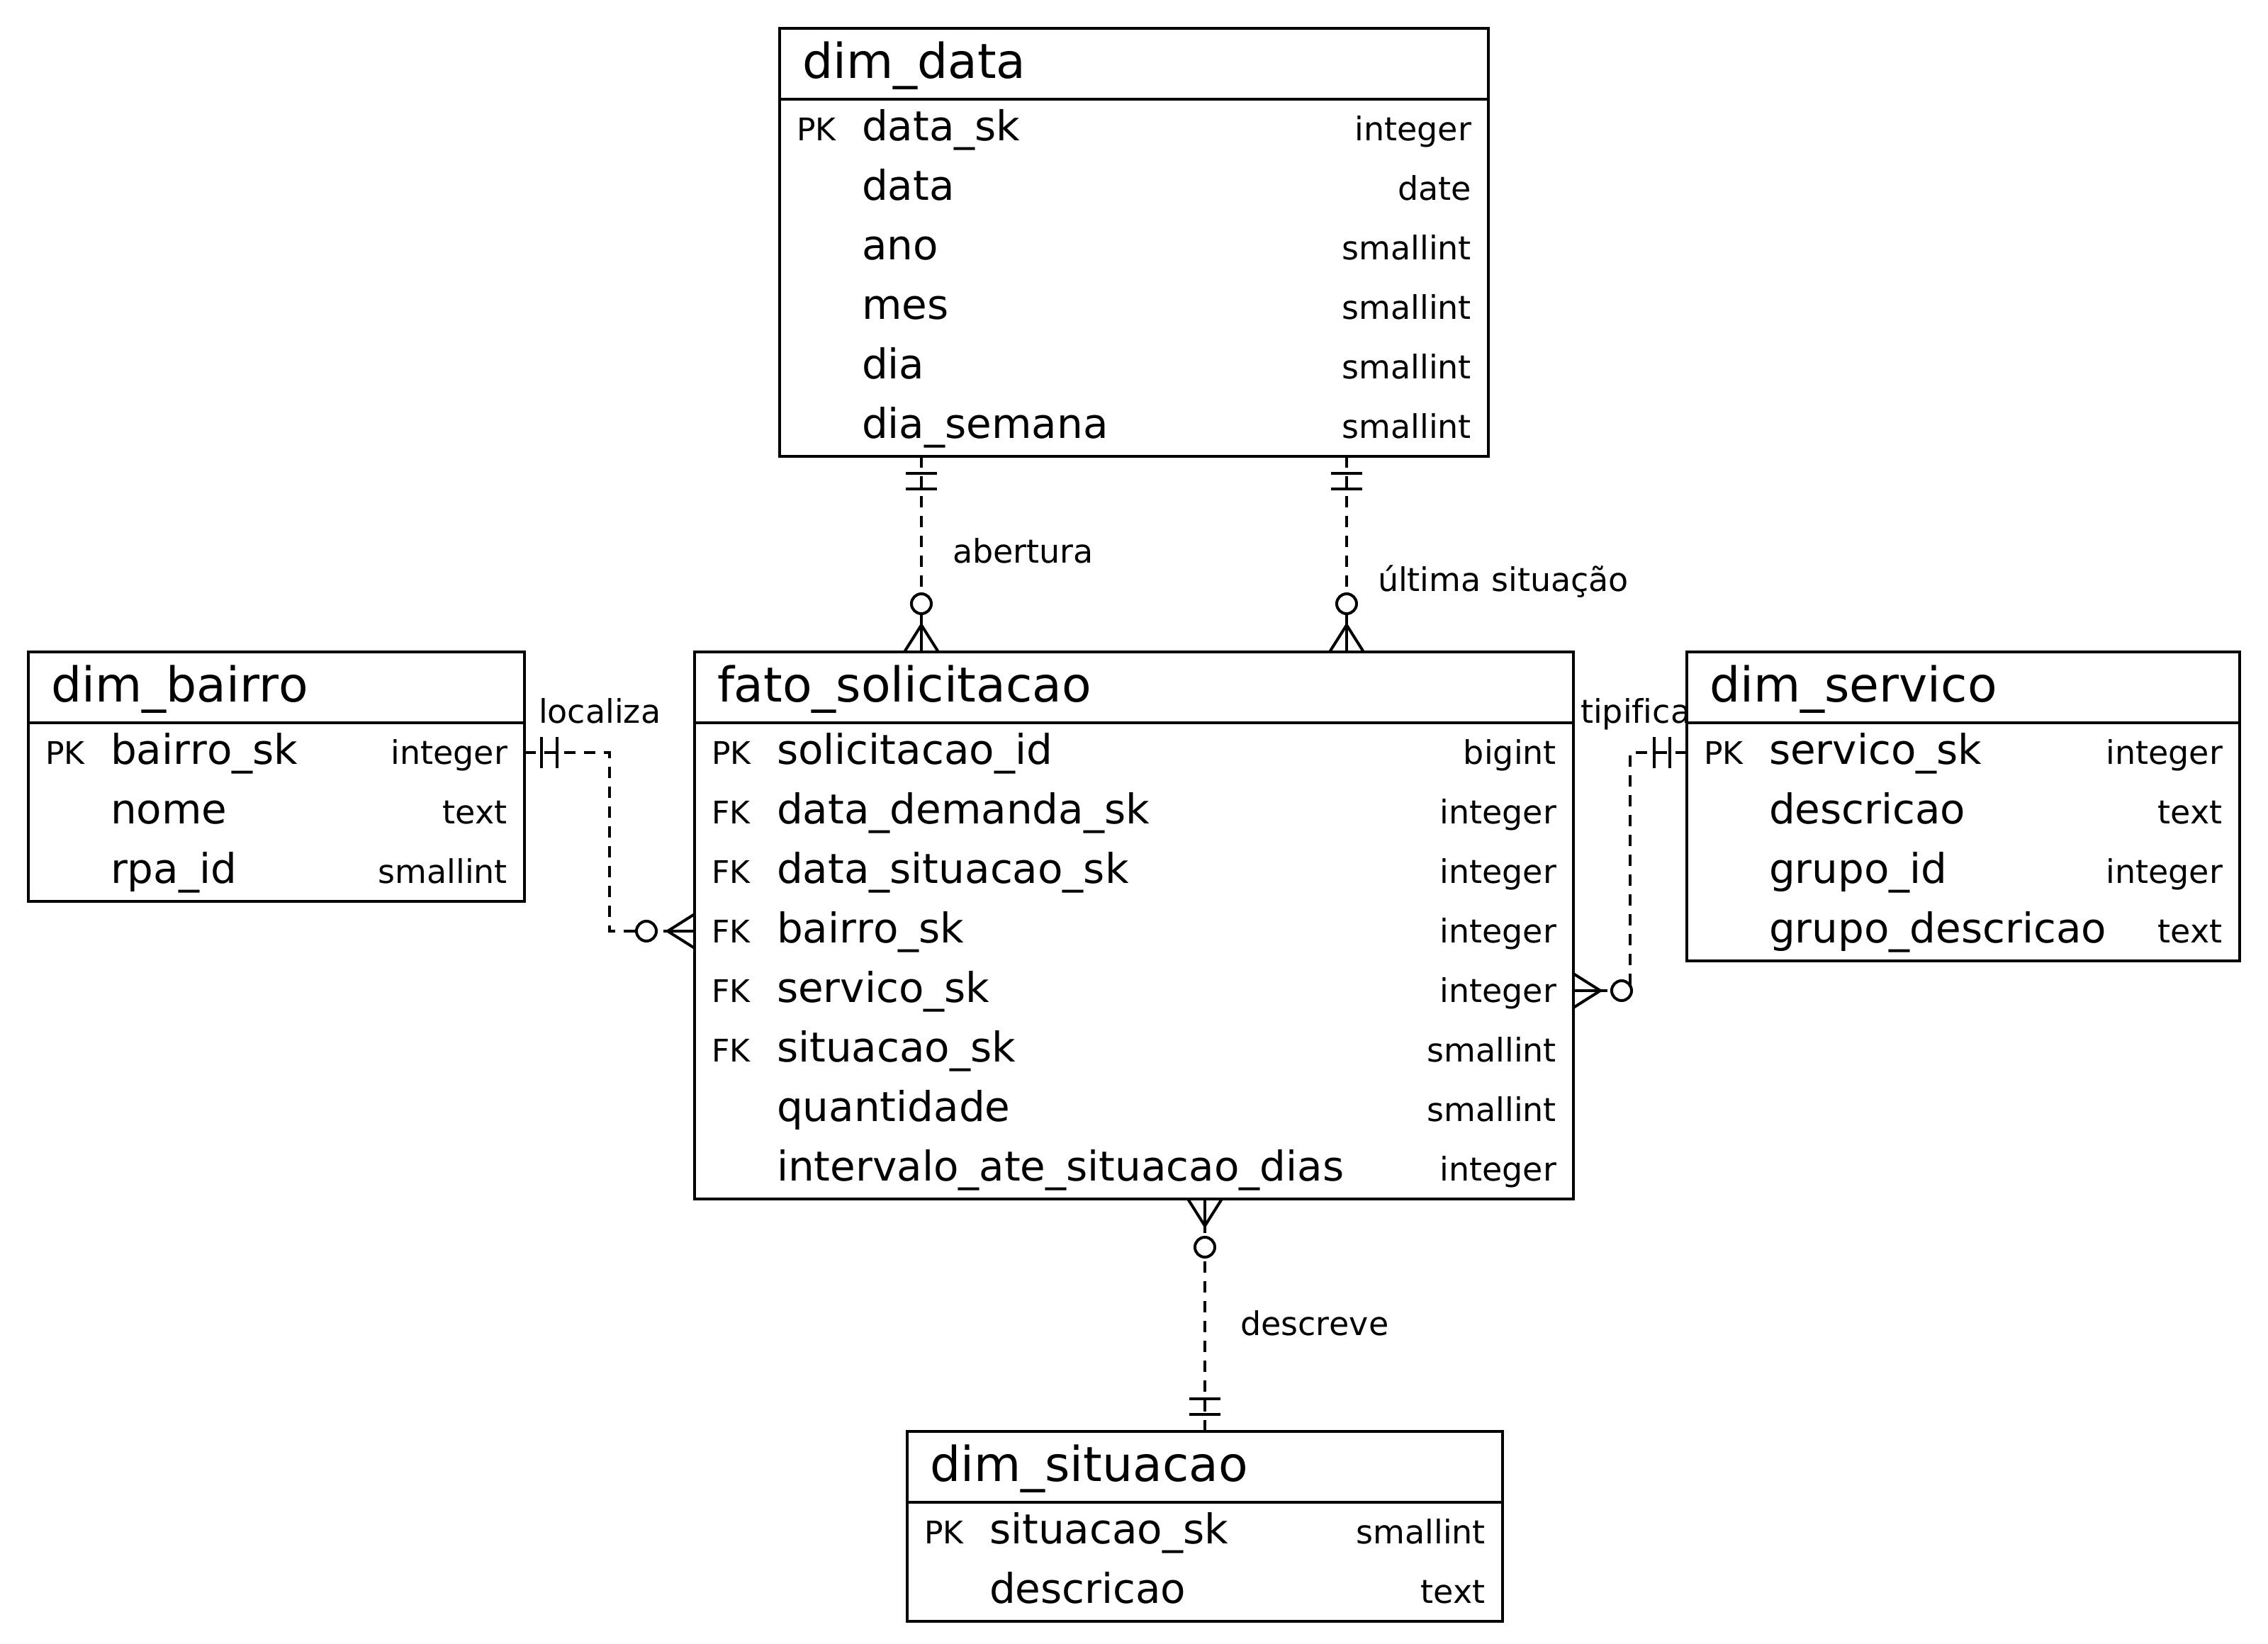
\includegraphics[width=0.78\textwidth]{../docs/diagrams/olap_model.png}
\caption{DER do modelo OLAP com duas relações para a dimensão de data.}\label{fig:olap}
\end{figure}

\section{Implementação e validação}

No tratamento dos dados, os espaços das extremidades dos textos foram retirados, os códigos oficiais de RPA, grupo e serviço foram mantidos e os bairros e as situações receberam chaves locais. Os valores ausentes, por sua vez, permaneceram sem preenchimento, e os registros no mesmo endereço foram mantidos. As coordenadas, entretanto, ficaram fora do modelo, porque faltam em 31.127 registros.

Em seguida, o roteiro SQL cria e carrega seis tabelas OLTP, quatro dimensões e uma tabela fato (Apêndice~B), cujas 42 colunas estão documentadas no dicionário de dados (Apêndice~A). A comparação entre os modelos, feita por identificador, chaves, datas e medida, não encontrou divergências. Além disso, os testes confirmaram a rejeição de PK duplicada, de FK inexistente e de última situação anterior à demanda, e a repetição da carga OLAP preservou o conteúdo.

Na versão analisada, 33.662 registros estão como ATENDIDA e 830 têm outras situações. Entre os registros ATENDIDA, a mediana do intervalo até esse status é de dois dias, embora haja datas de última situação até 10/09/2025, ou seja, posteriores ao fim do período de abertura.

\section{Dashboards}

As consultas foram organizadas em três níveis de decisão, com cinco consultas em cada um. O nível operacional atende a equipe de campo e a supervisão no dia a dia, o tático apoia a coordenação mês a mês, e o estratégico serve à direção da EMLURB e à prefeitura. Aquelas que dependem do tempo são relativas a uma data de referência, calculada na própria base como o último dia com abertura de chamado, de modo que expressões como ``últimos 7 dias'' e ``último mês'' se ajustam sozinhas quando a base é atualizada, e em operação essa data pode ser substituída pela data atual. As tabelas a seguir trazem o enunciado e o principal resultado de cada consulta, enquanto o código SQL completo está no Apêndice~C.

\begin{table}[H]
\centering\small
\caption{Consultas do nível operacional (data de referência: 31/08/2025).}
\begin{tabularx}{\textwidth}{lYY}
\toprule
\textbf{Q} & \textbf{Enunciado} & \textbf{Resultado principal} \\ \midrule
1 & Quais chamados não atendidos estão há mais tempo em aberto? & Os mais antigos estavam há 241 dias em aberto, quase todos do serviço de luminárias e com situação pendente. \\ \rowsep
2 & Quantos chamados não atendidos há em cada situação, por tempo em aberto? & Eram 830, e 306 dos 660 pendentes estavam há mais de 90 dias em aberto. \\ \rowsep
3 & Em quais bairros e serviços se acumulam os chamados não atendidos? & Brasília Teimosa lidera, com 61 chamados de luminárias não atendidos. \\ \rowsep
4 & Quais ruas tiveram três ou mais chamados nos últimos 30 dias? & A Av.\ Norte Miguel Arraes de Alencar, em Macaxeira, teve 52 chamados. \\ \rowsep
5 & Quantos chamados foram abertos por dia nos últimos 7 dias? & Foram 1.001, dos quais 74 ainda não constavam como atendidos. \\ \bottomrule
\end{tabularx}
\end{table}

\begin{table}[H]
\centering\small
\caption{Consultas do nível tático (data de referência: 31/08/2025).}
\begin{tabularx}{\textwidth}{lYY}
\toprule
\textbf{Q} & \textbf{Enunciado} & \textbf{Resultado principal} \\ \midrule
1 & Quantos chamados cada RPA abriu no último mês, em comparação com os meses anteriores? & No último mês (agosto de 2025), a RPA 6 ficou 15,1\% acima da sua média mensal. \\ \rowsep
2 & Quanto tempo cada serviço leva até o atendimento registrado? & Lâmpada apagada tem mediana de 2 dias, mas em luminárias 10\% levam mais de 63 dias. \\ \rowsep
3 & Que parcela dos chamados de cada mês foi atendida em até 7 dias? & Caiu de 97,2\% em janeiro para 93,3\% em junho. \\ \rowsep
4 & Quais bairros têm mais chamados? & Boa Viagem lidera, com 2.420 chamados. \\ \rowsep
5 & Em quais dias da semana chegam mais chamados? & Terça-feira tem a maior média (200 por dia), e sábado e domingo ficam abaixo de 70. \\ \bottomrule
\end{tabularx}
\end{table}

\begin{table}[H]
\centering\small
\caption{Consultas do nível estratégico (data de referência: 31/08/2025).}
\begin{tabularx}{\textwidth}{lYY}
\toprule
\textbf{Q} & \textbf{Enunciado} & \textbf{Resultado principal} \\ \midrule
1 & Como as seis RPAs se comparam em volume e atendimento? & A RPA 6 tem 23,7\% dos chamados e o menor percentual atendido (96,4\%). \\ \rowsep
2 & O número de chamados está crescendo? & Não na cidade como um todo: a média ficou entre 130 e 154 chamados por dia em todos os meses. \\ \rowsep
3 & Os chamados se concentram em poucos bairros? & Sim: os 10 bairros com mais chamados, de 93, somam 37,7\% do total. \\ \rowsep
4 & Quais tipos de serviço são mais pedidos? & Lâmpada apagada (75,9\%) e circuito apagado (17,6\%) somam 93,5\% dos chamados. \\ \rowsep
5 & Quanto tempo cada RPA leva para atender? & Nas RPAs 2 e 3, mais de 98\% dos chamados são atendidos em até 3 dias, e nas RPAs 4 a 6, cerca de 73\%. \\ \bottomrule
\end{tabularx}
\end{table}

\section{Mineração de dados}

\subsection{Problema}

As consultas mostram que os chamados se concentram em poucos bairros e se repetem nas mesmas ruas. Diante disso, o problema definido para a mineração foi decidir quais bairros e ruas devem receber manutenção preventiva primeiro e em que momento. Para respondê-lo, foram usados dois métodos complementares: o k-means descreve o perfil de cada bairro, ao passo que uma rede neural estima, para cada rua, a chance de nova solicitação nos dias seguintes.

\subsection{Perfis de bairros com k-means}

O k-means [MacQueen 1967] separa os itens em \textit{k} grupos sem precisar de rótulos prévios. Neste trabalho, cada bairro é representado por sete indicadores calculados no período, que são o volume de solicitações, a mediana e o percentil 90 de dias até o atendimento registrado, o percentual não atendido, o percentual de solicitações em ruas com chamados repetidos, o percentual de circuitos apagados e o percentual de danos na estrutura, como luminárias, postes e vãos de rede. Antes do agrupamento, os indicadores passam por z-score, para que nenhum deles domine os demais apenas por causa da escala.

O algoritmo sorteia \textit{k} centros, atribui cada bairro ao centro mais próximo e recalcula cada centro como a média dos seus bairros, repetindo esses passos até que os grupos parem de mudar. Como o resultado depende do sorteio inicial, o processo foi executado 20 vezes, mantendo-se a solução mais compacta. Entre 2 e 8 grupos, o valor \textit{k}~=~4 obteve a maior silhueta e, por isso, foi adotado. A Tabela~\ref{tab:kmeans} resume os perfis encontrados, e a Figura~\ref{fig:kmeans} mostra o centro de cada grupo.

\begin{table}[H]
\centering\small
\caption{Perfis de bairros encontrados pelo k-means.}\label{tab:kmeans}
\begin{tabularx}{\textwidth}{lYcY}
\toprule
\textbf{Grupo} & \textbf{Perfil} & \textbf{Bairros} & \textbf{Exemplos} \\ \midrule
1 & Alta demanda e atendimento mais lento, reunindo 67\% dos chamados & 39 & Boa Viagem, Santo Amaro, Boa Vista \\ \rowsep
2 & Atendimento rápido e mais circuitos apagados que os demais grupos & 26 & Guabiraba, Macaxeira, Casa Amarela \\ \rowsep
3 & Baixa demanda e mais pendências & 23 & Nova Descoberta, Vasco da Gama, Água Fria \\ \rowsep
4 & Baixa demanda e mais danos na estrutura que os demais grupos & 5 & Ilha Joana Bezerra, Coelhos, Coqueiral \\ \bottomrule
\end{tabularx}
\end{table}

\begin{figure}[H]
\centering
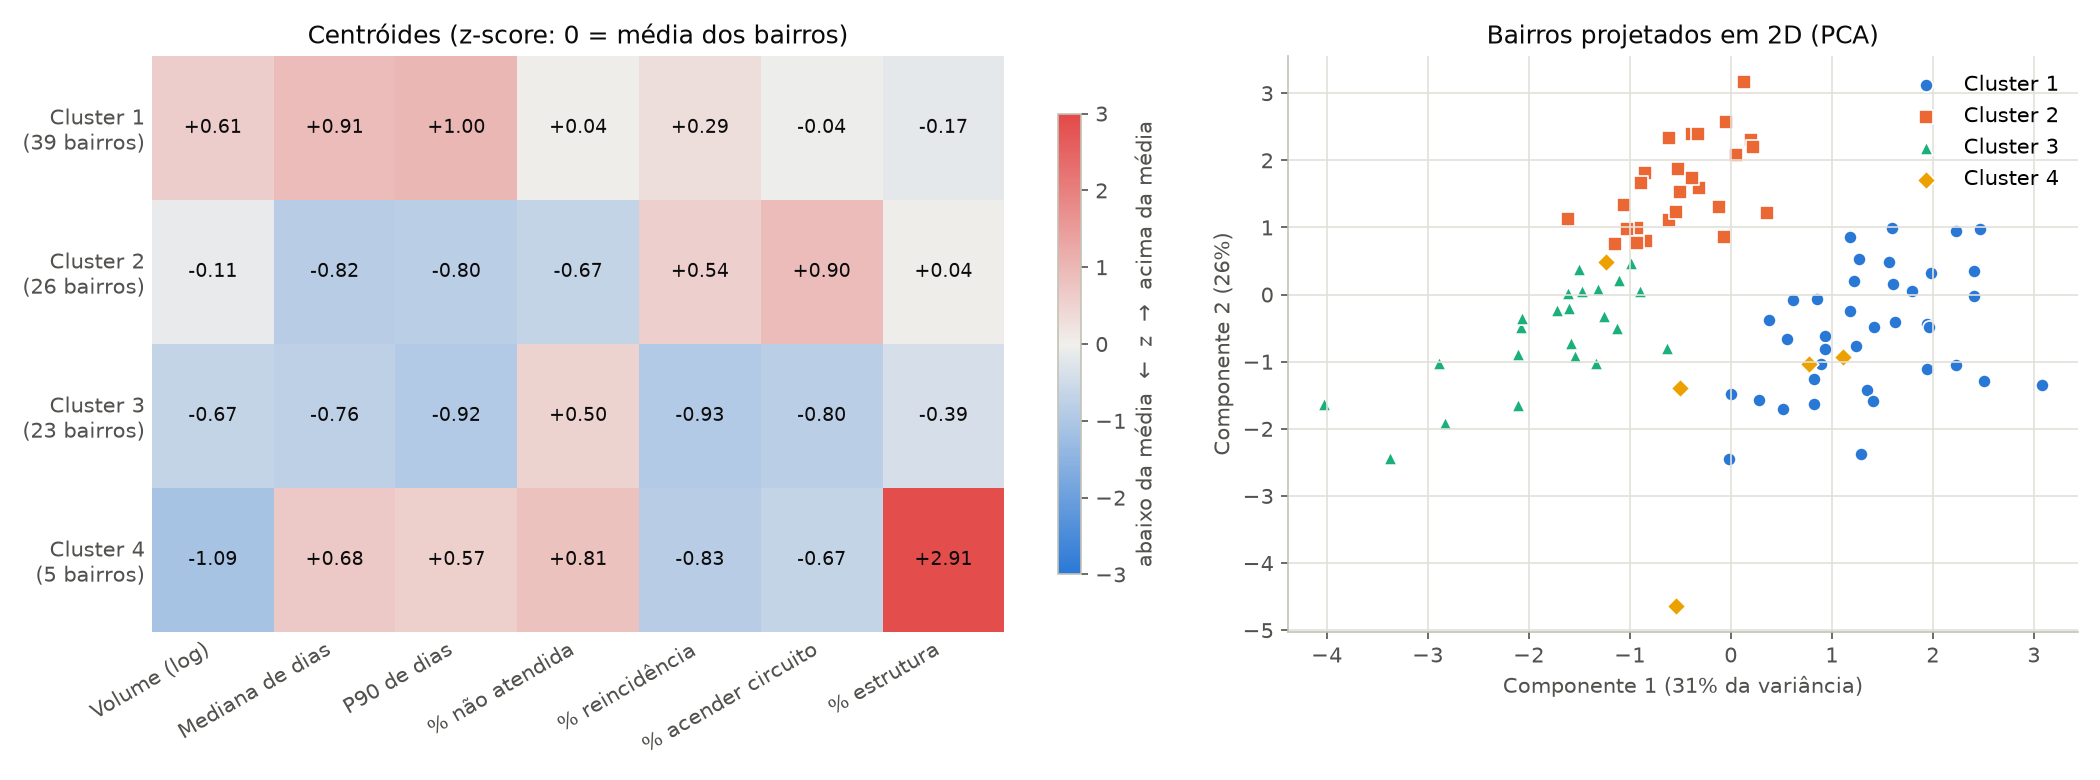
\includegraphics[width=\textwidth]{../docs/analysis/kmeans_profiles.png}
\caption{Centros dos grupos em z-score (à esquerda) e bairros projetados em duas dimensões (à direita).}\label{fig:kmeans}
\end{figure}

\subsection{Prioridade das ruas com rede neural}

Na análise por rua, a unidade é definida pelo bairro e pelo logradouro, já que essa é a menor unidade que os dados permitem acompanhar. Para cada rua e cada mês de corte, a rede recebe 15 entradas calculadas nos três meses anteriores ao corte: o número de solicitações, os meses com solicitação, os dias desde a última, o percentual ainda aberto no corte, os percentuais de circuitos apagados e de danos na estrutura, a mediana de dias até o atendimento, a quantidade de números de imóvel distintos e a RPA. Assim como no k-means, essas entradas passam por z-score.

Como saída, a rede estima a chance de a rua ter nova solicitação até 7, 14, 21, 31, 45 e 62 dias após o corte. Para isso, ela tem duas camadas ocultas, de 32 e 16 neurônios, e uma saída para cada um desses prazos, seguindo o modelo proposto por Gensheimer e Narasimhan [2019]. Esse modelo também aproveita as ruas cujo prazo ainda não havia terminado quando os dados acabam, já que as considera sem solicitação apenas até ali, sem supor o que ocorreu depois. Por fim, o treino usou os cortes de abril a julho de 2025, ao passo que o teste usou o corte de agosto, que a rede não havia visto.

No teste, 92\% das 200 ruas com maior risco previsto tiveram nova solicitação em até 31 dias, enquanto a média entre as 3.540 ruas avaliadas foi de 32\%.

Em seguida, as ruas foram agrupadas com k-means, a partir da chance prevista em cada prazo, em três tipos, chamados de crônico, recorrente e esporádico (Tabela~\ref{tab:tipos}). Nos três tipos, a chance prevista ficou próxima do que de fato ocorreu em agosto. Além disso, como mostra a Figura~\ref{fig:tipos}, as ruas crônicas, embora sejam apenas 9\% do total, concentraram 36\% das solicitações da primeira semana. Aplicada ao corte de setembro de 2025, a rede indicou 328 ruas crônicas e 857 recorrentes, que formam a base do plano de ação.

\begin{table}[H]
\centering\small
\caption{Tipos de rua definidos pela rede neural (teste de agosto de 2025).}\label{tab:tipos}
\begin{tabularx}{\textwidth}{lcccY}
\toprule
\textbf{Tipo} & \textbf{Ruas} & \textbf{Previsto em 31 dias} & \textbf{Ocorrido em 31 dias} & \textbf{Perfil típico} \\ \midrule
Crônica & 325 (9\%) & 86\% & 85\% & 12 chamados no trimestre, o último há 3 dias \\ \rowsep
Recorrente & 937 (26\%) & 49\% & 41\% & 4 chamados, o último há 16 dias \\ \rowsep
Esporádica & 2.278 (64\%) & 23\% & 21\% & 1 chamado, há 46 dias \\ \bottomrule
\end{tabularx}
\end{table}

\begin{figure}[H]
\centering
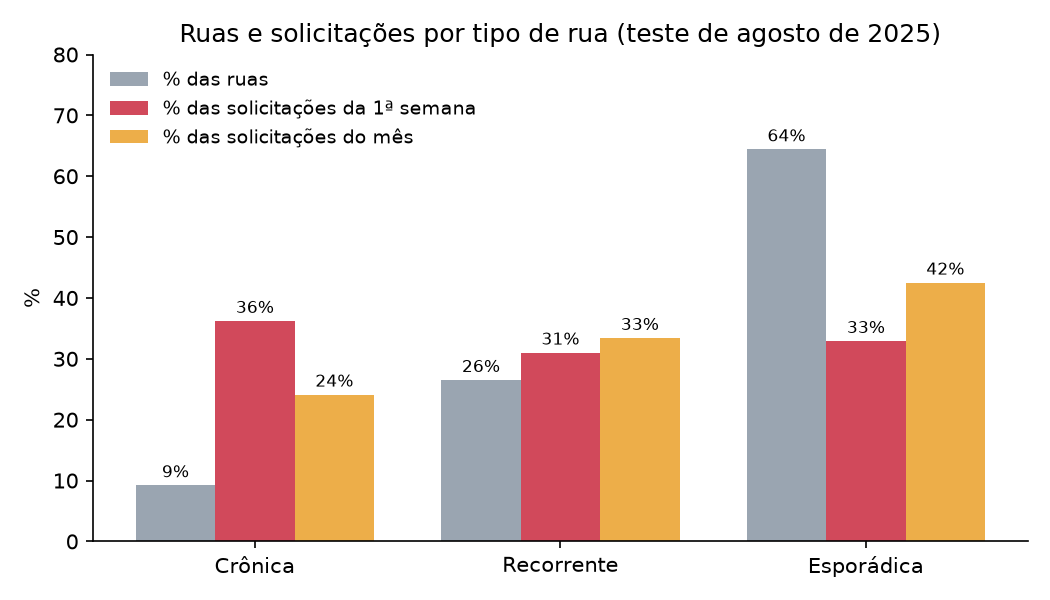
\includegraphics[width=0.72\textwidth]{../docs/analysis/street_types.png}
\caption{Participação de cada tipo de rua no total de ruas e nas solicitações do teste.}\label{fig:tipos}
\end{figure}

\section{Plano de ação 5W2H}

O plano tem um único objetivo, que é reduzir os chamados repetidos de iluminação agindo antes de o cidadão reclamar. Esse objetivo é tratado em três escalas, que correspondem aos níveis dos dashboards, de modo que cada coluna da Tabela~\ref{tab:5w2h} representa uma ação completa.

\begin{table}[H]
\centering\small
\caption{Plano de ação 5W2H.}\label{tab:5w2h}
\begin{tabularx}{\textwidth}{L{1.6cm}YYY}
\toprule
 & \textbf{Operacional: rua} & \textbf{Tático: bairro} & \textbf{Estratégico: cidade} \\ \midrule
\textbf{What} & Inspecionar as 328 ruas crônicas apontadas pela rede neural (ex.: Av.\ Norte Miguel Arraes de Alencar, Av.\ Agamenon Magalhães) & Revisar os circuitos dos 26 bairros do grupo ``circuitos apagados'' do k-means (ex.: Guabiraba, Macaxeira, Casa Amarela) & Adotar a lista mensal de ruas prioritárias como rotina da EMLURB \\ \rowsep
\textbf{Why} & Essas ruas são 9\% do total, mas geraram mais de 1/3 dos chamados da primeira semana$^{1}$ & Nesses bairros, 1 em cada 4 chamados é de trecho inteiro apagado$^{2}$, enquanto na cidade é 1 em 6$^{3}$ & A rede neural acertou 92\% das 200 ruas que indicou como prioritárias$^{1}$ \\ \rowsep
\textbf{Where} & Ruas da lista do mês (a primeira, de setembro de 2025) & Principalmente RPAs 2 e 3 & Toda a cidade, começando pela RPA 6, onde os chamados mais cresceram$^{4}$ \\ \rowsep
\textbf{When} & Toda primeira semana do mês & A cada trimestre & A partir do próximo ano \\ \rowsep
\textbf{Who} & Equipe de campo & Coordenação de iluminação & Direção da EMLURB \\ \rowsep
\textbf{How} & Vistoria preventiva de lâmpadas e circuito & Checar relés e alimentação dos trechos que apagam & Gerar a lista todo mês e cadastrar os postes \\ \rowsep
\textbf{How much} & Tempo das equipes já existentes & Equipe de rede elétrica e troca de peças quando necessário & Cadastro dos postes (investimento único) \\ \bottomrule
\end{tabularx}
\par\vspace{3pt}
\begin{minipage}{\textwidth}\footnotesize
Origem dos dados: $^{1}$rede neural (Seção 6.3), $^{2}$k-means de bairros (Seção 6.2), $^{3}$consulta estratégica Q4 e $^{4}$consulta tática Q1.
\end{minipage}
\end{table}

\section*{Referências}
\begin{list}{}{\leftmargin=0.6cm\itemindent=-0.6cm\itemsep=3pt\parsep=0pt}
\small
\item Emlurb (2026). Sobre. Autarquia de Manutenção e Limpeza Urbana do Recife. \url{https://emlurb.recife.pe.gov.br/sobre-0}. Acesso em 18 out. 2026.
\item Gensheimer, M. F. e Narasimhan, B. (2019). A scalable discrete-time survival model for neural networks. \textit{PeerJ}, 7:e6257.
\item Instituto de Pesquisa Econômica Aplicada (Ipea) (2026). ODS 11: Cidades e comunidades sustentáveis. \url{https://www.ipea.gov.br/ods/ods11.html}. Acesso em 18 out. 2026.
\item MacQueen, J. (1967). Some methods for classification and analysis of multivariate observations. In \textit{Proceedings of the Fifth Berkeley Symposium on Mathematical Statistics and Probability}, v. 1, p. 281--297.
\item Recife (2026). Central de Atendimento de Serviços da EMLURB 156. Recurso 2025, Prefeitura do Recife. \url{https://dados.recife.pe.gov.br/dataset/central-de-atendimento-de-servicos-da-emlurb-156}. Acesso em 18 out. 2026.
\end{list}

\clearpage
\appendix
\renewcommand{\thesection}{\Alph{section}}
\titleformat{\section}{\fontsize{13}{15}\selectfont\bfseries}{Apêndice \thesection.}{0.4em}{}

\section{Dicionário de dados}

Todas as colunas são obrigatórias (NOT NULL). PK indica chave primária e FK, chave estrangeira.

{\small
\begin{longtable}{L{4.5cm}L{1.7cm}L{7.0cm}}
\toprule
\textbf{Coluna} & \textbf{Tipo} & \textbf{Definição e regra} \\ \midrule
\endhead
\multicolumn{3}{l}{\textbf{oltp.rpa}} \\ \rowsep
rpa\_id & smallint & PK. Código oficial da RPA, de 1 a 6. \\ \rowsep
\multicolumn{3}{l}{\textbf{oltp.bairro}} \\ \rowsep
bairro\_id & integer & PK. Chave local da combinação RPA e nome. \\ \rowsep
rpa\_id & smallint & FK para oltp.rpa. \\ \rowsep
nome & text & Nome publicado, não vazio. Único por RPA. \\ \rowsep
\multicolumn{3}{l}{\textbf{oltp.grupo\_servico}} \\ \rowsep
grupo\_id & integer & PK. Código oficial do grupo (4 no recorte). \\ \rowsep
descricao & text & Descrição oficial do grupo, não vazia. \\ \rowsep
\multicolumn{3}{l}{\textbf{oltp.servico}} \\ \rowsep
servico\_id & integer & PK. Código oficial do serviço. \\ \rowsep
grupo\_id & integer & FK para oltp.grupo\_servico. \\ \rowsep
descricao & text & Descrição oficial do serviço, não vazia. \\ \rowsep
\multicolumn{3}{l}{\textbf{oltp.situacao}} \\ \rowsep
situacao\_id & smallint & PK. Chave local da situação. \\ \rowsep
descricao & text & Última situação publicada. Única e não vazia. \\ \rowsep
\multicolumn{3}{l}{\textbf{oltp.solicitacao}} \\ \rowsep
solicitacao\_id & bigint & PK, maior que zero. Número da linha no CSV original, que não é protocolo oficial. \\ \rowsep
bairro\_id & integer & FK para oltp.bairro. \\ \rowsep
servico\_id & integer & FK para oltp.servico. \\ \rowsep
situacao\_id & smallint & FK para oltp.situacao. \\ \rowsep
logradouro & text & Logradouro publicado. Não identifica um poste. \\ \rowsep
numero & text & Número publicado, mantido como texto. \\ \rowsep
data\_demanda & date & Data de abertura, de 01/01 a 31/08/2025. \\ \rowsep
data\_ultima\_situacao & date & Data do último status, igual ou posterior à abertura. \\ \rowsep
\multicolumn{3}{l}{\textbf{olap.dim\_data}} \\ \rowsep
data\_sk & integer & PK. Data no formato AAAAMMDD. \\ \rowsep
data & date & Data do calendário. Única. \\ \rowsep
ano & smallint & Ano civil. \\ \rowsep
mes & smallint & Mês, de 1 a 12. \\ \rowsep
dia & smallint & Dia do mês, de 1 a 31. \\ \rowsep
dia\_semana & smallint & Dia da semana ISO: segunda = 1, domingo = 7. \\ \rowsep
\multicolumn{3}{l}{\textbf{olap.dim\_bairro}} \\ \rowsep
bairro\_sk & integer & PK. Igual à chave local do bairro. \\ \rowsep
nome & text & Nome do bairro. \\ \rowsep
rpa\_id & smallint & RPA do bairro (atributo desnormalizado). \\ \rowsep
\multicolumn{3}{l}{\textbf{olap.dim\_servico}} \\ \rowsep
servico\_sk & integer & PK. Igual ao código oficial do serviço. \\ \rowsep
descricao & text & Descrição do serviço. \\ \rowsep
grupo\_id & integer & Código do grupo (desnormalizado). \\ \rowsep
grupo\_descricao & text & Descrição do grupo (desnormalizada). \\ \rowsep
\multicolumn{3}{l}{\textbf{olap.dim\_situacao}} \\ \rowsep
situacao\_sk & smallint & PK. Igual à chave local da situação. \\ \rowsep
descricao & text & Situação publicada. Única. \\ \rowsep
\multicolumn{3}{l}{\textbf{olap.fato\_solicitacao}} \\ \rowsep
solicitacao\_id & bigint & PK. Dimensão degenerada, igual à chave do OLTP. \\ \rowsep
data\_demanda\_sk & integer & FK para olap.dim\_data, no papel de data de abertura. \\ \rowsep
data\_situacao\_sk & integer & FK para olap.dim\_data, no papel de data da última situação. \\ \rowsep
bairro\_sk & integer & FK para olap.dim\_bairro. \\ \rowsep
servico\_sk & integer & FK para olap.dim\_servico. \\ \rowsep
situacao\_sk & smallint & FK para olap.dim\_situacao. \\ \rowsep
quantidade & smallint & Medida aditiva, sempre 1. Conta registros, não postes. \\ \rowsep
intervalo\_ate\_situacao\_dias & integer & Dias entre a abertura e a última situação, maior ou igual a zero. Indica prazo de atendimento apenas em ATENDIDA. \\ \bottomrule
\end{longtable}
}

\section{Script de construção dos ambientes OLTP e OLAP}

\begin{lstlisting}
BEGIN;
CREATE SCHEMA oltp;
CREATE TABLE oltp.rpa (
 rpa_id smallint PRIMARY KEY CHECK (rpa_id BETWEEN 1 AND 6)
);
CREATE TABLE oltp.bairro (
 bairro_id integer PRIMARY KEY,
 rpa_id smallint NOT NULL REFERENCES oltp.rpa,
 nome text NOT NULL CHECK (btrim(nome) <> ''),
 UNIQUE (rpa_id, nome)
);
CREATE TABLE oltp.grupo_servico (
 grupo_id integer PRIMARY KEY,
 descricao text NOT NULL CHECK (btrim(descricao) <> '')
);
CREATE TABLE oltp.servico (
 servico_id integer PRIMARY KEY,
 grupo_id integer NOT NULL REFERENCES oltp.grupo_servico,
 descricao text NOT NULL CHECK (btrim(descricao) <> '')
);
CREATE TABLE oltp.situacao (
 situacao_id smallint PRIMARY KEY,
 descricao text NOT NULL UNIQUE CHECK (btrim(descricao) <> '')
);
CREATE TABLE oltp.solicitacao (
 solicitacao_id bigint PRIMARY KEY CHECK (solicitacao_id > 0),
 bairro_id integer NOT NULL REFERENCES oltp.bairro,
 servico_id integer NOT NULL REFERENCES oltp.servico,
 situacao_id smallint NOT NULL REFERENCES oltp.situacao,
 logradouro text NOT NULL,
 numero text NOT NULL,
 data_demanda date NOT NULL,
 data_ultima_situacao date NOT NULL CHECK (data_ultima_situacao >= data_demanda)
);
COMMENT ON COLUMN oltp.solicitacao.solicitacao_id IS 'Identifica a linha do CSV original desta versão. Não corresponde ao protocolo municipal.';
COMMENT ON COLUMN oltp.solicitacao.data_ultima_situacao IS 'Registra a data do último status publicado. A fonte não informa o histórico nem garante que essa seja a data do reparo.';
CREATE INDEX ON oltp.solicitacao (bairro_id, data_demanda);
CREATE INDEX ON oltp.solicitacao (servico_id);
CREATE INDEX ON oltp.solicitacao (situacao_id);
COMMIT;
BEGIN;
CREATE SCHEMA olap;
CREATE TABLE olap.dim_data (
 data_sk integer PRIMARY KEY,
 data date NOT NULL UNIQUE,
 ano smallint NOT NULL,
 mes smallint NOT NULL CHECK (mes BETWEEN 1 AND 12),
 dia smallint NOT NULL CHECK (dia BETWEEN 1 AND 31),
 dia_semana smallint NOT NULL CHECK (dia_semana BETWEEN 1 AND 7)
);
CREATE TABLE olap.dim_bairro (
 bairro_sk integer PRIMARY KEY,
 nome text NOT NULL,
 rpa_id smallint NOT NULL
);
CREATE TABLE olap.dim_servico (
 servico_sk integer PRIMARY KEY,
 descricao text NOT NULL,
 grupo_id integer NOT NULL,
 grupo_descricao text NOT NULL
);
CREATE TABLE olap.dim_situacao (
 situacao_sk smallint PRIMARY KEY,
 descricao text NOT NULL UNIQUE
);
CREATE TABLE olap.fato_solicitacao (
 solicitacao_id bigint PRIMARY KEY,
 data_demanda_sk integer NOT NULL REFERENCES olap.dim_data,
 data_situacao_sk integer NOT NULL REFERENCES olap.dim_data,
 bairro_sk integer NOT NULL REFERENCES olap.dim_bairro,
 servico_sk integer NOT NULL REFERENCES olap.dim_servico,
 situacao_sk smallint NOT NULL REFERENCES olap.dim_situacao,
 quantidade smallint NOT NULL DEFAULT 1 CHECK (quantidade = 1),
 intervalo_ate_situacao_dias integer NOT NULL CHECK (intervalo_ate_situacao_dias >= 0)
);
COMMENT ON COLUMN olap.fato_solicitacao.intervalo_ate_situacao_dias IS 'Conta os dias entre a demanda e a última situação. Em ATENDIDA, indica o intervalo até o atendimento registrado. Não mede a duração física do reparo.';
COMMIT;
\end{lstlisting}

\clearpage
\section{Código das consultas}

Nas consultas que dependem do tempo, \texttt{ref} calcula a data de referência como o último dia com abertura na base. Em operação, ela pode ser trocada por \texttt{CURRENT\_DATE}.

\subsection*{Nível operacional}
\noindent\begin{minipage}{\textwidth}
\small\textbf{Q1.} Quais chamados não atendidos estão há mais tempo em aberto?\par\vspace{2pt}
\begin{lstlisting}
WITH ref AS (SELECT max(d.data) AS hoje FROM olap.fato_solicitacao f JOIN olap.dim_data d ON d.data_sk=f.data_demanda_sk)
SELECT f.solicitacao_id,b.nome AS bairro,b.rpa_id,sv.descricao AS servico,st.descricao AS situacao,
 dd.data AS abertura,ds.data AS ultima_situacao,ref.hoje-dd.data AS dias_em_aberto
 FROM olap.fato_solicitacao f CROSS JOIN ref
 JOIN olap.dim_situacao st ON st.situacao_sk=f.situacao_sk
 JOIN olap.dim_bairro b ON b.bairro_sk=f.bairro_sk
 JOIN olap.dim_servico sv ON sv.servico_sk=f.servico_sk
 JOIN olap.dim_data dd ON dd.data_sk=f.data_demanda_sk
 JOIN olap.dim_data ds ON ds.data_sk=f.data_situacao_sk
 WHERE st.descricao<>'ATENDIDA'
 ORDER BY dias_em_aberto DESC,f.solicitacao_id LIMIT 15;
\end{lstlisting}
\end{minipage}\par\vspace{8pt}
\noindent\begin{minipage}{\textwidth}
\small\textbf{Q2.} Quantos chamados não atendidos há em cada situação, por tempo em aberto?\par\vspace{2pt}
\begin{lstlisting}
WITH ref AS (SELECT max(d.data) AS hoje FROM olap.fato_solicitacao f JOIN olap.dim_data d ON d.data_sk=f.data_demanda_sk)
SELECT st.descricao AS situacao,
 count(*) FILTER (WHERE ref.hoje-dd.data<=30) AS ate_30_dias,
 count(*) FILTER (WHERE ref.hoje-dd.data BETWEEN 31 AND 90) AS de_31_a_90,
 count(*) FILTER (WHERE ref.hoje-dd.data BETWEEN 91 AND 180) AS de_91_a_180,
 count(*) FILTER (WHERE ref.hoje-dd.data>180) AS acima_180,
 count(*) AS total
 FROM olap.fato_solicitacao f CROSS JOIN ref
 JOIN olap.dim_situacao st ON st.situacao_sk=f.situacao_sk
 JOIN olap.dim_data dd ON dd.data_sk=f.data_demanda_sk
 WHERE st.descricao<>'ATENDIDA'
 GROUP BY st.descricao ORDER BY total DESC;
\end{lstlisting}
\end{minipage}\par\vspace{8pt}
\noindent\begin{minipage}{\textwidth}
\small\textbf{Q3.} Em quais bairros e serviços se acumulam os chamados não atendidos?\par\vspace{2pt}
\begin{lstlisting}
SELECT b.nome AS bairro,b.rpa_id,sv.descricao AS servico,count(*) AS nao_atendidos,
 min(dd.data) AS abertura_mais_antiga
 FROM olap.fato_solicitacao f
 JOIN olap.dim_situacao st ON st.situacao_sk=f.situacao_sk
 JOIN olap.dim_bairro b ON b.bairro_sk=f.bairro_sk
 JOIN olap.dim_servico sv ON sv.servico_sk=f.servico_sk
 JOIN olap.dim_data dd ON dd.data_sk=f.data_demanda_sk
 WHERE st.descricao<>'ATENDIDA'
 GROUP BY b.nome,b.rpa_id,sv.descricao ORDER BY nao_atendidos DESC,bairro LIMIT 15;
\end{lstlisting}
\end{minipage}\par\vspace{8pt}
\noindent\begin{minipage}{\textwidth}
\small\textbf{Q4.} Quais ruas tiveram três ou mais chamados nos últimos 30 dias?\par\vspace{2pt}
\begin{lstlisting}
WITH ref AS (SELECT max(data_demanda) AS hoje FROM oltp.solicitacao)
SELECT s.logradouro,b.nome AS bairro,count(*) AS chamados,
 count(*) FILTER (WHERE st.descricao<>'ATENDIDA') AS nao_atendidos,
 min(s.data_demanda) AS primeiro,max(s.data_demanda) AS ultimo
 FROM oltp.solicitacao s CROSS JOIN ref
 JOIN oltp.bairro b ON b.bairro_id=s.bairro_id
 JOIN oltp.situacao st ON st.situacao_id=s.situacao_id
 WHERE s.data_demanda>ref.hoje-30
 GROUP BY s.logradouro,b.nome HAVING count(*)>=3
 ORDER BY chamados DESC,nao_atendidos DESC,s.logradouro LIMIT 15;
\end{lstlisting}
\end{minipage}\par\vspace{8pt}
\noindent\begin{minipage}{\textwidth}
\small\textbf{Q5.} Quantos chamados foram abertos por dia nos últimos 7 dias?\par\vspace{2pt}
\begin{lstlisting}
WITH ref AS (SELECT max(d.data) AS hoje FROM olap.fato_solicitacao f JOIN olap.dim_data d ON d.data_sk=f.data_demanda_sk)
SELECT dd.data,dd.dia_semana,count(*) AS abertos,
 count(*) FILTER (WHERE st.descricao='ATENDIDA') AS atendidos,
 count(*) FILTER (WHERE st.descricao<>'ATENDIDA') AS nao_atendidos
 FROM olap.fato_solicitacao f CROSS JOIN ref
 JOIN olap.dim_situacao st ON st.situacao_sk=f.situacao_sk
 JOIN olap.dim_data dd ON dd.data_sk=f.data_demanda_sk
 WHERE dd.data>ref.hoje-7
 GROUP BY dd.data,dd.dia_semana ORDER BY dd.data;
\end{lstlisting}
\end{minipage}\par\vspace{8pt}

\subsection*{Nível tático}
\noindent\begin{minipage}{\textwidth}
\small\textbf{Q1.} Quantos chamados cada RPA abriu no último mês, em comparação com os meses anteriores?\par\vspace{2pt}
\begin{lstlisting}
WITH ref AS (SELECT date_trunc('month',max(d.data))::date AS mes_atual
  FROM olap.fato_solicitacao f JOIN olap.dim_data d ON d.data_sk=f.data_demanda_sk),
m AS (SELECT b.rpa_id,date_trunc('month',d.data)::date AS mes,count(*) AS chamados
  FROM olap.fato_solicitacao f
  JOIN olap.dim_bairro b ON b.bairro_sk=f.bairro_sk
  JOIN olap.dim_data d ON d.data_sk=f.data_demanda_sk
  GROUP BY b.rpa_id,date_trunc('month',d.data))
SELECT m.rpa_id,
 sum(m.chamados) FILTER (WHERE m.mes=ref.mes_atual) AS ultimo_mes,
 round(avg(m.chamados) FILTER (WHERE m.mes<ref.mes_atual),1) AS media_meses_anteriores,
 round(100.0*sum(m.chamados) FILTER (WHERE m.mes=ref.mes_atual)
  /avg(m.chamados) FILTER (WHERE m.mes<ref.mes_atual)-100,1) AS variacao_pct
 FROM m CROSS JOIN ref
 GROUP BY m.rpa_id ORDER BY variacao_pct DESC;
\end{lstlisting}
\end{minipage}\par\vspace{8pt}
\noindent\begin{minipage}{\textwidth}
\small\textbf{Q2.} Quanto tempo cada serviço leva até o atendimento registrado?\par\vspace{2pt}
\begin{lstlisting}
SELECT sv.descricao AS servico,count(*) AS atendidos,
 percentile_disc(0.5) WITHIN GROUP (ORDER BY f.intervalo_ate_situacao_dias) AS mediana_dias,
 percentile_disc(0.9) WITHIN GROUP (ORDER BY f.intervalo_ate_situacao_dias) AS p90_dias,
 round(avg(f.intervalo_ate_situacao_dias),1) AS media_dias
 FROM olap.fato_solicitacao f
 JOIN olap.dim_situacao st ON st.situacao_sk=f.situacao_sk
 JOIN olap.dim_servico sv ON sv.servico_sk=f.servico_sk
 WHERE st.descricao='ATENDIDA'
 GROUP BY sv.descricao ORDER BY atendidos DESC;
\end{lstlisting}
\end{minipage}\par\vspace{8pt}
\noindent\begin{minipage}{\textwidth}
\small\textbf{Q3.} Que parcela dos chamados de cada mês foi atendida em até 7 dias?\par\vspace{2pt}
\begin{lstlisting}
SELECT d.mes,count(*) AS abertos,
 round(100.0*count(*) FILTER (WHERE st.descricao='ATENDIDA')/count(*),1) AS pct_atendida,
 round(100.0*count(*) FILTER (WHERE st.descricao='ATENDIDA' AND f.intervalo_ate_situacao_dias<=7)/count(*),1) AS pct_atendida_ate_7_dias
 FROM olap.fato_solicitacao f
 JOIN olap.dim_situacao st ON st.situacao_sk=f.situacao_sk
 JOIN olap.dim_data d ON d.data_sk=f.data_demanda_sk
 GROUP BY d.mes ORDER BY d.mes;
\end{lstlisting}
\end{minipage}\par\vspace{8pt}
\noindent\begin{minipage}{\textwidth}
\small\textbf{Q4.} Quais bairros têm mais chamados?\par\vspace{2pt}
\begin{lstlisting}
SELECT rank() OVER (ORDER BY count(*) DESC) AS posicao,b.nome AS bairro,b.rpa_id,count(*) AS chamados,
 round(100.0*count(*)/sum(count(*)) OVER (PARTITION BY b.rpa_id),1) AS pct_da_rpa
 FROM olap.fato_solicitacao f
 JOIN olap.dim_bairro b ON b.bairro_sk=f.bairro_sk
 GROUP BY b.nome,b.rpa_id ORDER BY chamados DESC LIMIT 15;
\end{lstlisting}
\end{minipage}\par\vspace{8pt}
\noindent\begin{minipage}{\textwidth}
\small\textbf{Q5.} Em quais dias da semana chegam mais chamados?\par\vspace{2pt}
\begin{lstlisting}
SELECT d.dia_semana,count(DISTINCT d.data) AS dias,count(*) AS chamados,
 round(count(*)::numeric/count(DISTINCT d.data),1) AS media_por_dia
 FROM olap.fato_solicitacao f
 JOIN olap.dim_data d ON d.data_sk=f.data_demanda_sk
 GROUP BY d.dia_semana ORDER BY d.dia_semana;
\end{lstlisting}
\end{minipage}\par\vspace{8pt}

\subsection*{Nível estratégico}
\noindent\begin{minipage}{\textwidth}
\small\textbf{Q1.} Como as seis RPAs se comparam em volume e atendimento?\par\vspace{2pt}
\begin{lstlisting}
SELECT b.rpa_id,count(DISTINCT b.bairro_sk) AS bairros,count(*) AS chamados,
 round(100.0*count(*)/sum(count(*)) OVER (),1) AS pct_do_total,
 round(count(*)::numeric/count(DISTINCT b.bairro_sk),0) AS chamados_por_bairro,
 round(100.0*count(*) FILTER (WHERE st.descricao='ATENDIDA')/count(*),1) AS pct_atendida
 FROM olap.fato_solicitacao f
 JOIN olap.dim_bairro b ON b.bairro_sk=f.bairro_sk
 JOIN olap.dim_situacao st ON st.situacao_sk=f.situacao_sk
 GROUP BY b.rpa_id ORDER BY chamados DESC;
\end{lstlisting}
\end{minipage}\par\vspace{8pt}
\noindent\begin{minipage}{\textwidth}
\small\textbf{Q2.} O número de chamados está crescendo?\par\vspace{2pt}
\begin{lstlisting}
SELECT d.mes,count(*) AS chamados,count(DISTINCT d.data) AS dias,
 round(count(*)::numeric/count(DISTINCT d.data),1) AS media_diaria,
 round(100.0*(count(*)::numeric/count(DISTINCT d.data))
  /lag(count(*)::numeric/count(DISTINCT d.data)) OVER (ORDER BY d.mes)-100,1) AS var_media_diaria_pct
 FROM olap.fato_solicitacao f
 JOIN olap.dim_data d ON d.data_sk=f.data_demanda_sk
 GROUP BY d.mes ORDER BY d.mes;
\end{lstlisting}
\end{minipage}\par\vspace{8pt}
\noindent\begin{minipage}{\textwidth}
\small\textbf{Q3.} Os chamados se concentram em poucos bairros?\par\vspace{2pt}
\begin{lstlisting}
WITH r AS (
 SELECT b.bairro_sk,count(*) AS chamados,row_number() OVER (ORDER BY count(*) DESC) AS posicao
 FROM olap.fato_solicitacao f JOIN olap.dim_bairro b ON b.bairro_sk=f.bairro_sk
 GROUP BY b.bairro_sk)
SELECT faixa,count(*) AS bairros,sum(chamados) AS chamados,
 round(100.0*sum(chamados)/(SELECT sum(chamados) FROM r),1) AS pct_chamados
 FROM (SELECT chamados,CASE WHEN posicao<=10 THEN '1. top 10' WHEN posicao<=30 THEN '2. 11 a 30'
  ELSE '3. demais' END AS faixa FROM r) x
 GROUP BY faixa ORDER BY faixa;
\end{lstlisting}
\end{minipage}\par\vspace{8pt}
\noindent\begin{minipage}{\textwidth}
\small\textbf{Q4.} Quais tipos de serviço são mais pedidos?\par\vspace{2pt}
\begin{lstlisting}
SELECT sv.descricao AS servico,count(*) AS chamados,
 round(100.0*count(*)/sum(count(*)) OVER (),1) AS pct_do_total,
 round(100.0*count(*) FILTER (WHERE st.descricao='ATENDIDA')/count(*),1) AS pct_atendida,
 count(*) FILTER (WHERE st.descricao<>'ATENDIDA') AS nao_atendidos
 FROM olap.fato_solicitacao f
 JOIN olap.dim_servico sv ON sv.servico_sk=f.servico_sk
 JOIN olap.dim_situacao st ON st.situacao_sk=f.situacao_sk
 GROUP BY sv.descricao ORDER BY chamados DESC;
\end{lstlisting}
\end{minipage}\par\vspace{8pt}
\noindent\begin{minipage}{\textwidth}
\small\textbf{Q5.} Quanto tempo cada RPA leva para atender?\par\vspace{2pt}
\begin{lstlisting}
SELECT b.rpa_id,count(*) AS atendidos,
 percentile_disc(0.5) WITHIN GROUP (ORDER BY f.intervalo_ate_situacao_dias) AS p50_dias,
 percentile_disc(0.75) WITHIN GROUP (ORDER BY f.intervalo_ate_situacao_dias) AS p75_dias,
 percentile_disc(0.9) WITHIN GROUP (ORDER BY f.intervalo_ate_situacao_dias) AS p90_dias,
 round(100.0*count(*) FILTER (WHERE f.intervalo_ate_situacao_dias<=3)/count(*),1) AS pct_ate_3_dias
 FROM olap.fato_solicitacao f
 JOIN olap.dim_situacao st ON st.situacao_sk=f.situacao_sk
 JOIN olap.dim_bairro b ON b.bairro_sk=f.bairro_sk
 WHERE st.descricao='ATENDIDA'
 GROUP BY b.rpa_id ORDER BY b.rpa_id;
\end{lstlisting}
\end{minipage}\par\vspace{8pt}

\end{document}
